\section{Tricycle drive}

The Tricycle setup defines the kinematics of AGV as follows: it features a single actuated and steerable wheel along with two additional passive wheels. 
Independent control of $\theta$ is not possible unless $\alpha(t)$ can achieve up to 90 degrees. 
Additionally, the Instantaneous Center of Curvature (ICC) must align with the line passing through the fixed wheels.
\begin{figure}[H]
    \centering
    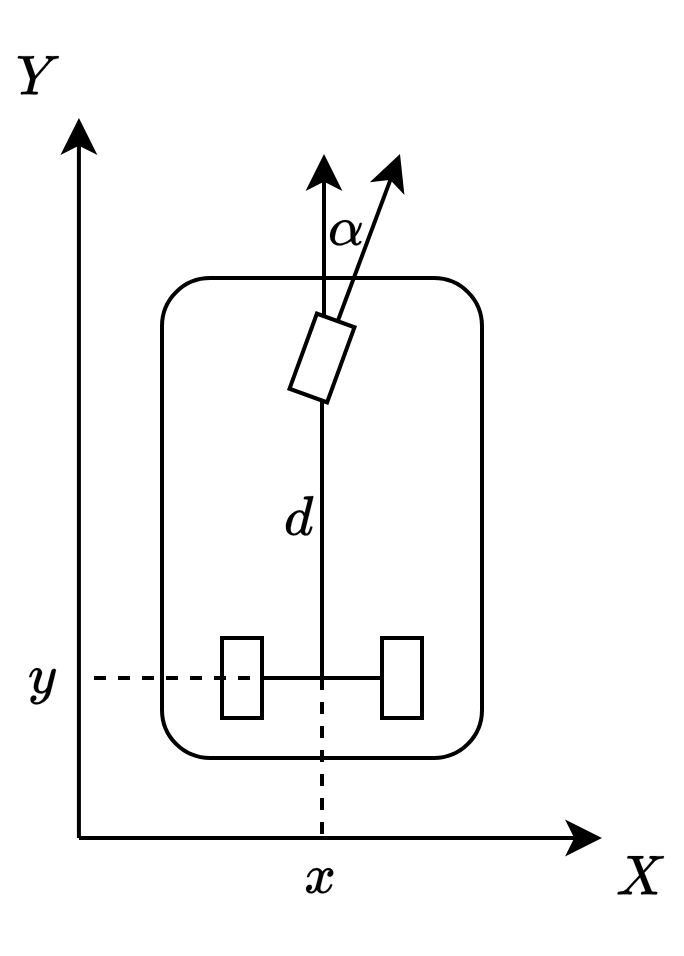
\includegraphics[width=0.3\linewidth]{images/td.png} 
    \caption{Tricycle drive robot}
\end{figure}
The robot's control parameters consist of the steering direction $\alpha(t)$ the angular velocity of the steering wheel $\omega_s(t)$. 

In this configuration, when $\alpha(t)=0$ and $\omega_s(t)=\omega$ at a specific time instant, the robot moves linearly. 
Conversely, when $\alpha(t)=90^\circ$ and $\omega(t)=\omega$ at a particular time instant, the robot rotates in place. 

\subsection{Odometry}
The direct kinematics can be derived as follows: 
\[\begin{cases}
    r = \text{steering wheel radius} \\
    V_S(t)=\omega_S(t)r \\
    R(t)=d\tan\left(\dfrac{\pi}{2}-\alpha(t)\right) \\
    \omega(t)=\dfrac{\omega_s(t)r}{\sqrt{d^2+R(t)^2}}=\frac{V_S(t)}{d}\sin\alpha
\end{cases}\]
In the base frame: 
\[\begin{cases}
    \dot{x}(t)=V_S(t)\cos\alpha(t)+\cos\theta(t)=V(t)\cos\theta(t) \\
    \dot{y}(t)=V_S(t)\cos\alpha(t)+\cos\theta(t)=V(t)\sin\theta(t) \\
    \dot{\theta}=\dfrac{V_S(t)}{d}\sin\alpha(t)=\omega(t)
\end{cases}\]